\documentclass[a4paper,12pt]{article}
\usepackage{extsizes}

%\usepackage[T2A]{fontenc}
%\usepackage[utf8x]{inputenc}
\usepackage[TS1,T2A]{fontenc}
\usepackage[utf8]{inputenc}
\usepackage[english,russian]{babel}
\usepackage{tikz}
\usepackage[european,cuteinductors,smartlabels]{circuitikz}

\usepackage{amsmath,amsfonts}
\usepackage{amssymb}
\usepackage[scr]{rsfso}

\usepackage{gnuplottex}


%%% Межстрочный интервал
\usepackage{setspace}

%% таблицы
\usepackage{booktabs}

%% для кода
\usepackage{color}
\usepackage{listingsutf8}

\definecolor{lightgrey}{rgb}{0.9,0.9,0.9}
\definecolor{lightblue}{rgb}{0,0,1}

\definecolor{grey}{rgb}{0.5,0.5,0.5}
\definecolor{blue}{rgb}{0,0,1}
\definecolor{violet}{rgb}{0.5,0,0.5}

\definecolor{darkred}{rgb}{0.5,0,0}
\definecolor{darkblue}{rgb}{0,0,0.5}
\definecolor{darkgreen}{rgb}{0,0.5,0}


\lstset{%
  language=C++,%
  morekeywords={constexpr,nullptr,size_t,uint32_t,assert,override,final},%
  basicstyle=\ttfamily\footnotesize,%
  sensitive=true,%
  keywordstyle=\color{blue},%
  stringstyle=\color{darkgreen},%
  commentstyle=\color{violet},%
  showstringspaces=false,%
  tabsize=2,%
  frame=leftline,
  rulecolor=\color{lightblue},
  xleftmargin=10pt,
}

\lstset{
%extendedchars=\true,
%inputencoding=utf8x,   
  numberstyle=\tiny,
  numbers=left,
  numbersep=10pt,
  xleftmargin=10pt,
  %framesep=4.5mm,
  %framexleftmargin=2.5mm,
  framexleftmargin=5pt,
  framesep=15pt,
  fillcolor=\color{lightgrey},
}


\title{Повышающий преобразователь}
\author{}
% Конец преамбулы
\begin{document}
%\maketitle
%\begin{tikzpicture}
%\newcommand{\xb}{-3}
%\newcommand{\xa}{3}
%\draw[thin, ->] (-6,0) -- (6,0) node[right] {$X$};
%\draw[thin, ->] (0,-6) -- (0,6) node[left] {$Y$};
%\foreach \x\xtext in {-5/-5,5/5,{\xb}/\xb,{\xa}/{\displaystyle \frac{-b+\sqrt{b^2-4ac}}{2a}}} % 
%   \draw (\x,0.1) -- (\x,-0.1) node[below] {$\xtext$};

 %\draw[domain=-5:5, help lines, smooth]
 %       plot ({\x},{0.2*(\x-\xa)*(\x-\xb)});
%\end{tikzpicture}


\section{Повышающий преобразователь}

\begin{figure}[!ht]
\centering
\begin{tikzpicture}
        \draw(0,3) to[L,l=L,o-] (3,3) -- (6,3) to [C,l_=C] (6,0) to[short,-o] (0,0);
	\draw(4,3) to[short] (8.5,3) to[R,l_=R] (8.5,0) to [short] (6,0);
	\draw(3,0) to[cosw,l_=SW] (3,3);
	\draw (3,3) to[D-,l=D] (6,3);
        \draw[->,>=latex] (9.2,2.1) -- (9.2,0.9) node[midway,right] {$i_1$};
        \draw[->,>=latex] (6.7,2.1) -- (6.7,0.9) node[midway,right] {$i_2$};
        \draw (0,1.5) node {$U_1$};
\end{tikzpicture}
\caption{повышающий преобразователь}
\end{figure}

Рассмотрим работу преобразователя в двух стадиях:

\subsection{стадия I}
\begin{figure}[!ht]
\centering
\begin{tikzpicture}
	\draw(0,3) to[L,l=L,o-] (3,3) -- (4,3) to [C,l_=C] (4,0) to[short,-o] (0,0);
	\draw(4,3) to[short,*-] (6.5,3) to[R,l_=R] (6.5,0) to [short,-*] (4,0);
	\draw[->,>=latex] (7.2,2.1) -- (7.2,0.9) node[midway,right] {$i_1$};
	\draw[->,>=latex] (4.7,2.1) -- (4.7,0.9) node[midway,right] {$i_2$};
	\draw (0,1.5) node {$U_1$};
\end{tikzpicture}
\caption{стадия I работы повышающего преобразователя}
\end{figure}
At t=0 we have $i_1(0) = i_{10}$ and $i_2(0) = i_{20}$.
$$
U=const
$$
Lets get graphs for $i_1(t), i_2(t)$ from analitic solution of differencial equations for the circuit.

\begin{equation}
\left\{
\begin{array}{lll}
U_1 = L\frac{\partial i}{\partial t} + R i_1 & \Rightarrow & 0 = L\frac{\partial^2 i}{\partial t^2} + R \frac{\partial i_1}{\partial t} \\
	U_1 = L\frac{\partial i}{\partial t} + \frac{1}{C}\int\limits_0^t i_2(\tau) d\tau & \Rightarrow & 0 = L\frac{\partial^2 i}{\partial t^2} + \frac{1}{C} i_2
\end{array}
\right.
\label{initial}
\end{equation}

Из первого и второго уравнения системы (\ref{initial}) получаем:

\begin{equation}
R\frac{\partial i_1}{\partial t} = \frac{1}{C} i_2 \Rightarrow \frac{\partial i_1}{\partial t} = \frac{1}{RC} i_2 
\label{first}
\end{equation}

из первого уравнения системы (\ref{initial}), учитываем $i_1(t) + i_2(t) = i(t)$:

$$
\frac{\partial i_1}{\partial t} + \frac{\partial i_2}{\partial t} = -\frac{R}{L} i_1 + \frac{U_1}{L} 
$$

%Сведем систему 2-х уравнений первого порядка к одному уравнению второго порядка (исключаем $i_2$):

%$$
%\frac{\partial i_1}{\partial t} + RC\frac{\partial^2 i_1}{\partial t^2} = -\frac{R}{L} i_1 + \frac{U_1}{L}
%$$

%Решение есть сумма общего решения однородного уравнения
%$$
%RC\frac{\partial^2 i_1}{\partial t^2} +  \frac{\partial i_1}{\partial t}  + \frac{R}{L} i_1 = 0
%$$
%и частного решения неоднородного (с ненулевой правой частью).







В этом уравнении заменим $\frac{\partial i_1}{\partial t}$ из (\ref{first}):

$$
\frac{\partial i_2}{\partial t} = - \frac{R}{L} i_1 - \frac{1}{RC} i_2 + \frac{U_1}{L}
$$

\begin{equation}
\frac{\partial}{\partial t}\!\left(\begin{array}{c}i_1\\[1.5mm]i_2\end{array}\right) =
	\left(\begin{array}{cc}0&\frac{1}{RC}\\[1.5mm] -\frac{R}{L}&-\frac{1}{RC}\end{array}\right)
		\left(\begin{array}{c}i_1\\[1.5mm]i_2\end{array}\right)
		+
	\left(\begin{array}{c}0\\[1.5mm]\frac{U_1}{L}\end{array}\right)
\end{equation}

Предполагая решение в виде $i(t) = e^{\lambda t}$ получаем характеристическое уравнение.

$$
\left(\begin{array}{cc}-\lambda & \frac{1}{RC}\\[1.5mm] -\frac{R}{L} & -\lambda -\frac{1}{RC}\end{array}\right) =0  \Rightarrow \lambda^2 + \lambda \frac{1}{RC} + \frac{1}{LC} =0
$$

$$
D = b^2 - 4ac = \frac{1}{(RC)^2} - \frac{4}{LC}
$$

$$
\lambda_{1,2} = \frac{-b \pm \sqrt{D}}{2a} = -\frac{1}{2RC} \pm \sqrt{\frac{1}{(2RC)^2}- \frac{1}{LC}}
= -\alpha \pm j\omega
$$

$$
i_1(t) = A\cdot e^{\lambda_1 t} + B\cdot e^{\lambda_2 t} + \frac{U_1}{R}
$$
$$
i_2(t) = \left(A\cdot \lambda_1e^{\lambda_1 t} + B\cdot \lambda_2e^{\lambda_2 t}\right)\frac{1}{2\alpha}
$$



При $t=0$ получаем:

$$
A + B + \frac{U_1}{R} = i_{10}
$$
$$
\lambda_1 \cdot A + \lambda_2 \cdot B = i_{20}\cdot2\alpha
$$



Для определения коэффициентов получаем матрицу
$$
\left(
\begin{array}{cc}
  1 & 1 \\[1.5mm] 
  \lambda_1 & \lambda_2 
\end{array}
\right)\left(
\begin{array}{c}
  A\\[1.5mm]
  B 
\end{array}  
\right)=\left(
\begin{array}{c}
	i_1(0) - \frac{U_1}{R}\\[1.5mm]
  i_2(0) \cdot 2\alpha
\end{array}
\right)
$$
решая в Reduce-algebra
\lstinputlisting[linerange={1-3}]{AB.red}
$$
\begin{array}{ccl}
	A&=&-\frac{i_1(0)\lambda_2}{\lambda_1-\lambda_2} + \frac{i_2(0)\cdot2\alpha}{\lambda_1-\lambda_2} + \frac{\lambda_2}{\lambda_1-\lambda_2}\frac{U}{R}\\[1.5mm]
	B&=&\frac{i_1(0)\lambda_1}{\lambda_1-\lambda_2} - \frac{i_2(0)\cdot2\alpha}{\lambda_1-\lambda_2} - \frac{\lambda_1}{\lambda_1-\lambda_2}\frac{U}{R}
\end{array}
$$

упростим 
$$
\lambda_1 - \lambda_2 = \sqrt{\frac{1}{(RC)^2} - \frac{4}{LC}} = j \sqrt{\frac{4}{LC} - \frac{1}{(RC)^2}} = 2j\cdot \mathcal{I}m = 2j\omega
$$




еще три упрощения:
$$
\frac{\lambda_2e^{\lambda_1t} - \lambda_1e^{\lambda_2t}}{\lambda_1-\lambda_2} = -e^{-\alpha t}
\left(\cos(\omega t) + \frac{\alpha}{\omega} \sin(\omega t)\right)
$$

$$
\frac{e^{\lambda_1t} - e^{\lambda_2t}}{\lambda_1-\lambda_2} = e^{-\alpha t}
\frac{\sin\omega t}{\omega}
$$

$$
\frac{\lambda_1e^{\lambda_1t} - \lambda_2e^{\lambda_2t}}{\lambda_1-\lambda_2} = -e^{-\alpha t}
\left(\cos(\omega t) - \frac{\alpha}{\omega}\right)
$$

%%%  i_1
$$
i_1(t) = \frac{i_1(0) - \frac{U}{R}}{\lambda_1-\lambda_2} \left( -\lambda_2e^{\lambda_1 \cdot t}  + \lambda_1e^{\lambda_2 \cdot t} \right)
+\frac{i_2(0)2\alpha}{\lambda_1 - \lambda_2} \left(e^{\lambda_1\cdot t} - e^{\lambda_2\cdot t}\right)  + \frac{U}{R}=
$$

$$
= e^{-\alpha t} \left[ \left(i_1(0) - \frac{U}{R}\right)
\left(\cos(\omega t) + \frac{\alpha}{\omega} \sin(\omega t)\right)
+ i_2(0) \frac{\sin(\omega t)}{\omega} \right]  + \frac{U}{R} =
$$

$$
= \frac{e^{-\alpha t}}{\omega} \left[ \left(i_1(0) - \frac{U}{R}\right)
\left(\omega\cos(\omega t) + \alpha \sin(\omega t)\right)
+ i_2(0) \sin(\omega t) \right]  + \frac{U}{R}
$$


%%% i_2
$$
i_2(t) = RC\left\{-\alpha e^{-\alpha t} \left[ \left(i_1(0) - \frac{U}{R}\right)
\left(\cos(\omega t) + \frac{\alpha}{\omega} \sin(\omega t)\right)
+ i_2(0) \frac{2\alpha\cdot\sin(\omega t)}{\omega} \right]\right. +
$$
$$
+ \left.e^{-\alpha t} \left[  \left(i_1(0) - \frac{U}{R}\right) 
\left(-\omega\sin(\omega t) + \alpha \cos(\omega t)\right) + i_2(0)2\alpha\cos(\omega t)
\right]\right\} =
$$

$$
=  e^{-\alpha t} \frac{1}{2\alpha} \left[ \left(i_1(0) - \frac{U}{R}\right)
\left(-\omega - \frac{\alpha^2}{\omega}\right)\sin(\omega t) + 
i_2(0)\cdot 2\alpha\left(\cos(\omega t) - \frac{\alpha}{\omega}\sin(\omega t)\right)
\right] 
$$

здесь заметим, что 
$$
\alpha^2 + \omega^2 = \frac{1}{(2RC)^2} + \frac{1}{LC} - \frac{1}{(2RC)^2} = \frac{1}{LC}; \;\;\; 
\frac{1}{2\alpha} = RC; \;\;\;\; \frac{\alpha^2+\omega^2}{2a} = \frac{R}{L}
$$


$$
i_2(t)=\frac{e^{-\alpha t}}{\omega}
\left[ -\left(i_1(0) - \frac{U}{R}\right)\frac{R}{L}\sin(\omega t) 
+ i_2(0) \frac{1}{2\alpha} \left(\omega \cos(\omega t) - \alpha\sin(\omega t)\right)
\right] =
$$

$$
\frac{e^{-\alpha t}}{\omega}
\left[ -\left(i_1(0) - \frac{U}{R}\right)\frac{R}{L}\sin(\omega t)
+ i_2(0) RC \left(\omega \cos(\omega t) - \alpha\sin(\omega t)\right)
\right]
$$

Введем новые переменные ${\displaystyle \tilde{i}_1(t) = i_1(t) - \frac{U}{R}}$,
${\displaystyle \tilde{i}(t) = i(t) - \frac{U}{R}}$

тогда:
$$
\tilde{i}_1(t) = \frac{e^{-\alpha t}}{\omega} \left[ \tilde{i}_1(0) 
\left(\omega\cos(\omega t) + \alpha \sin(\omega t)\right)
+ i_2(0)\cdot 2\alpha \sin(\omega t) \right]
$$
$$
i_2(t)=\frac{e^{-\alpha t}}{\omega}
\left[ -\tilde{i}_1(0) \frac{\alpha^2+\omega^2}{2\alpha}\sin(\omega t) +
i_2(0) \left(\omega \cos(\omega t) - \alpha\sin(\omega t)\right)
\right]
$$

$$
\tilde{i}(t) = \frac{e^{-\alpha t}}{\omega} 
\left[
\omega	\tilde{i}_1(0)\left(\omega\cos(\omega t) + \frac{\alpha^2 - \omega^2}{2\alpha}\sin(\omega t) \right)
+ i_2(0)\left(\omega\cos(\omega t)  + \alpha\sin(\omega t)\right)
\right]
$$

% mathcal{Re}

%[  - i_10*l*lambda_2 + i_20*l + lambda_2*u ]
%[------------------------------------------]
%[         l*(lambda_1 - lambda_2)          ]
%[                                          ]
%[  i_10*l*lambda_1 - i_20*l - lambda_1*u   ]
%[ ---------------------------------------  ]
%[         l*(lambda_1 - lambda_2)          ]

Построить графики аналитического решения для токов $i_1(t)$, $i_2(t)$ и $i(t)$ с помощью программы {\bf gnuplot}. Пример построения в программе {\bf gnuplot}
представлен ниже:

\lstinputlisting{gnuplot.cmd}

Получить численное решение дифференциальных уравнений с помощью программы {\bf octave}. Пример численного решения в программе {\bf octave} представлен ниже:

\lstinputlisting{octave4.txt}

Смоделировать решение дифференциальных уравнений с помощью программы {\bf ngspice}. Пример моделирования решения с помощью {\bf ngspice} представлен ниже:

\lstinputlisting{check.cir}

Сравнить решения.

\subsection{стадия II}
\begin{figure}[!ht]
\centering
\begin{tikzpicture}
\draw(0,2) to [L,o-] (2,2) -- (2,0) to[short,-o] (0,0);
\draw ({4+0},0) to[C] ({4+0},2) -- ({4+2},2) to[R] ({4+2},0) -- ({4+0},0); 
\end{tikzpicture}
\caption{стадия II работы повышающего преобразователя}
\end{figure}

уравнение цепи на интервале $(n+\gamma)T \le t \le (n+1)T$

$$
RC \frac{d U_C}{dt} + U_C = 0
$$
%Введем новую переменную -- относительное время
%$$
%\bar{t} = \frac{t}{T}
%$$
%Введем новую переменную $\beta^{\prime\prime} = \frac{T}{RC}$

%тогда для уравнения
%$$
%\frac{1}{\beta^{\prime\prime}}\frac{dU_C}{dt} + U_C = 0
%$$

 для уравнения получаем решение
$$
U_C(t) = B_c e^{-\frac{1}{RC}t}
$$
аналогично для тока через резистор
$$
i_1(t) = i_1(n+\gamma) e^{-\frac{1}{RC}t}
$$

$$
i_1(n+1) = i_1(n+\gamma) e^{-\frac{1}{RC}(1-\gamma)\cdot T}
$$

для цепи с индуктивностью 
$$
U = L\frac{d i_L}{dt} 
$$
решение уравнения:
$$
i(t) = i(n+\gamma) + \frac{U}{L}\cdot t
$$


\subsection{Laplace way}

$$
\left\{
\begin{array}{lcl}
%	px - \frac{1}{RC} = 
	Li_1^\prime + L i_2^\prime + Rx &=& U\\[1.5mm]
	Li_1^\prime + L i_2^\prime + \frac{1}{C}\int i_2 d\tau &=& U
\end{array}
\right.
$$

$i_1^\prime, i_2^\prime $ -- производные по времени

$$
\left\{
\begin{array}{lcl}
	i_1^\prime &=& \frac{1}{RC} i_2\\[1.5mm]
	i_2^\prime &=& \frac{U}{L} - \frac{R}{L} i_1 - \frac{1}{RC} i_2
\end{array}
\right.
$$

Делаем замену
$$
\frac{U}{L} \doteqdot \frac{U}{L} \cdot \frac{1}{p};\; \; \; i_1 \doteqdot \tilde{I}_1 ;\; \; \; i_2 \doteqdot \tilde{I}_2; \; \; \;
i_1^\prime = \tilde{I}_1\cdot p - i_1(0); \; \; \;  i_2^\prime = p \tilde{I}_2 - i_2(0)
$$

$$
\left\{
	\begin{array}{lcl}
		p\cdot \tilde{I}_1 - i_1(0) &=& \frac{1}{RC} \cdot \tilde{I}_2\\[1.5mm]
		p\cdot \tilde{I}_2 - i_2(0) &=& \frac{U}{L}\cdot \frac{1}{p} - \frac{R}{L}\cdot \tilde{I}_1 -  \frac{1}{RC} \cdot \tilde{I}_2
	\end{array}
\right.
$$

$$
\left\{
\begin{array}{lcl}
	p\cdot I_1 - \frac{1}{RC}\cdot I_2& =& i_1(0)\\[1.5mm]
	\frac{R}{L}\cdot I_1 + \left( p + \frac{1}{RC}\right) I_2 &=& i_2(0) + \frac{U}{L}\cdot \frac{1}{p}
\end{array}
\right.
$$

$$
\Delta = \left| 
\begin{array}{cc} p          & -\frac{1}{RC} \\[1.5mm]
	\frac{R}{L} & p + \frac{1}{RC}
\end{array}\right| =
p\left(p + \frac{1}{RC}\right) = p^2 + \frac{1}{RC}\cdot p + \frac{1}{LC}=
p^2 +\frac{1}{RC}\cdot p + \frac{1}{LC} =
$$
$$
=p^2 + 2\cdot\frac{1}{2RC}p + \frac{1}{4R^2C^2} - \frac{1}{4R^2C^2} + \frac{1}{LC} =
\left(p+\frac{1}{2RC}\right)^2 - \frac{1}{4R^2C^2} \left( 1 - \frac{4R^2C}{L}\right) =
$$
$$
=\left(p + \frac{1}{2RC}\right)^2 + \frac{1}{4R^2C^2}\left(\frac{4R^2C}{L}-1\right)
$$

$$
\Delta_1 = \left|
\begin{array}{cc}
	i_1(0) & - \frac{1}{RC} \\[1.5mm]
	i_2(0) +\frac{U}{L}\cdot\frac{1}{p}& \left(p + \frac{1}{RC}\right) 
\end{array}
\right| =
i_1(0)\left(p + \frac{1}{RC}\right) + \frac{1}{RC}\left(i_2(0) + \frac{U}{L}\cdot {1}{p}\right) =
$$
$$
= \frac{1}{RC}(i_1(0) + i_2(0)) + i_1(0)\cdot p + \frac{U}{RLC} \cdot{1}{p} 
$$

$$
\Delta_2 = \left|
\begin{array}{cc} p          & i_1(0) \\[1.5mm]
\frac{R}{L} & i_2(0) + \frac{U}{L}\cdot\frac{1}{p}
\end{array}\right| = p\left(i_2(0)+\frac{U}{L}\cdot{1}{p}\right) - i_1(0)\frac{R}{L} =
i_2(0)p + \frac{U}{L} - \frac{R}{L}i_1(0)
$$


$$
I_1(p) = \frac{\frac{1}{RC}(i_1(0)+i_2(0)) + i_1(0)\cdot p + \frac{U}{RLC}\cdot \frac{1}{p}}
{\left(p + \frac{1}{2RC}\right)^2 + \frac{1}{4R^2C^2}\left(\frac{4R^2C}{L} - 1\right)}
$$

$$
I_2(p) = \frac{\frac{U}{L}- \frac{R}{L}i_1(0) + i_2(0)\cdot p}
{\left(p + \frac{1}{2RC}\right)^2 + \frac{1}{4R^2C^2}\left(\frac{4R^2C}{L} - 1\right)}
$$

разлагаем на множители знаменатель, и заменяем переменные
$$
\alpha = \frac{1}{2RC}; \omega = \frac{1}{2RC}\sqrt{\frac{4R^2C}{L}-1}
$$

$$
\Delta = \left(p + \frac{1}{2RC}\right)^2 + \frac{1}{4R^2C^2}\left(\frac{4R^2C}{L} - 1\right) =
(p+\alpha)^2 - (-1)\cdot\omega^2 =
$$
$$
=(p+\alpha)^2 - (j\cdot\omega)^2 = (p + \alpha - j\cdot\omega)(p+\alpha+j\cdot\omega)
$$
%$$
%\Delta_1 = i_1(0)(p + 2\alpha) + 2\alpha\left(i_2(0) + \frac{U}{L}\cdot\frac{1}{p}\right)
%$$

Разлагаем на множители по правилу:
$$
\xi p + \zeta = \frac{A}{p+a} + \frac{B}{p+b}
$$

если $p=-a$, то $-\xi a + \zeta = A(b-a)$

если $p=-b$, то $-\xi b + \zeta = B(b-a)$

В нашем случае:

$b=\alpha+i\omega; a = \alpha-i\omega; \xi = i_2(0); \zeta=\frac{U}{L}-\frac{R}{L} i_1(0) \Rightarrow$ 

$$
\zeta - \xi a = \frac{U}{L}-\frac{R}{L} i_1(0) - i_2(0)(\alpha-j\omega)
$$
$$
\zeta-\xi b = \frac{U}{L}-\frac{R}{L} i_1(0) - i_2(0)(\alpha + j\omega)
$$
$$
b-a = 2j\omega
$$

$$
I_2(p) = \frac{\frac{U}{L}- \frac{R}{L}i_1(0) + i_2(0)\cdot p}
{\left(p + \frac{1}{2RC}\right)^2 + \frac{1}{4R^2C^2}\left(\frac{4R^2C}{L} - 1\right)}=
\frac{\frac{U}{L}- \frac{R}{L}i_1(0) + i_2(0)\cdot p}{(p + \alpha - j\cdot\omega)(p+\alpha+j\cdot\omega)} =
$$
$$
=\frac{\frac{U}{L}-\frac{R}{L} i_1(0) - i_2(0)(\alpha-j\omega)}{2j\omega}
\frac{1}{(p + \alpha - j\omega)} -
\frac{\frac{U}{L}-\frac{R}{L} i_1(0) - i_2(0)(\alpha + j\omega)}{2j\omega}
\frac{1}{(p + \alpha + j\omega)}=
$$

$$
=\frac{\frac{U}{L}-\frac{R}{L} i_1(0) - i_2(0)\alpha}{2j\omega}
\left[\frac{1}{p+\alpha-j\omega} - \frac{1}{p+\alpha+j\omega} \right] + 
\frac{i_2(0)}{2}\left[\frac{1}{p+\alpha-j\omega} + \frac{1}{p+\alpha+j\omega} \right]
\doteqdot
$$
После обратного преобразования Лапласа

$$
\doteqdot
\frac{\frac{U}{L}-\frac{R}{L} i_1(0) - i_2(0)\alpha}{2j\omega}
\left[e^{-\alpha t}\cdot e^{j\omega t} - e^{-\alpha t}\cdot e^{-j\omega t}\right]
+\frac{i_2(0)}{2}\left[e^{-\alpha t}\cdot e^{j\omega t} + e^{-\alpha t}\cdot e^{-j\omega t}\right] =
$$
$$
= \frac{\left(\frac{U}{L}-\frac{R}{L} i_1(0) - i_2(0)\alpha\right)e^{-\alpha t}}{\omega} 
\left[\frac{e^{j\omega t} -  e^{-j \omega t}}{2j}\right] 
+ i_2(0) e^{-\alpha t} \left[\frac{e^{j\omega t} +  e^{-j \omega t}}{2}\right]
$$
$$
i_2(t) = \left[ \left(\frac{U}{L}-\frac{R}{L} i_1(0) - i_2(0)\alpha\right)\frac{\sin(\omega t)}{\omega}
+ i_2(0)\cos(\omega t) \right] e^{-\alpha t}
$$
заменяя координаты ${\displaystyle \tilde{i}_1(t) = i_1(t) - \frac{U}{R}}$, 
а также ${\displaystyle \frac{R}{L} = \frac{\alpha^2+\omega^2}{2\alpha}}$

$$
i_2(t) = e^{-\alpha t}\left[ \left(-\frac{\alpha^2+\omega^2}{2\alpha} \tilde{i}_1(0) - \alpha i_2(0)\right) 
\frac{\sin(\omega t)}{\omega} + i_2(0)\cos(\omega t)\right]
$$


$$
\frac{\partial}{\partial t}i_2(t) = -\alpha e^{-\alpha t}
\left[ \left(\frac{U}{L}-\frac{R}{L} i_1(0) - i_2(0)\alpha\right)\frac{\sin(\omega t)}{\omega}
+ i_2(0)\cos(\omega t) \right] +
$$
$$
+e^{-\alpha t} \left[\left(\frac{U}{L}-\frac{R}{L} i_1(0) - i_2(0)\alpha\right)\cos(\omega t) 
- i_2(0)\omega \sin(\omega t)\right] =
$$
$$
= e^{-\alpha t} \left[\left(-\left(\frac{U}{L} - \frac{R}{L}i_1(0) - \alpha i_2(0)\right) 
\frac{\alpha}{\omega} - i_2(0)\omega\right)\sin(\omega t)\right. +
$$
$$
+\left.\left(-\alpha i_2(0) + \frac{U}{L} - \frac{R}{L}i_1(0) - \alpha i_2(0) \right)\cos(\omega t)
\right]
$$

Из системы 
$$
\left\{
\begin{array}{lcl}
	L(i_1^\prime + i_2^\prime) + Ri_1 = U\\[1.5mm]
	i_1^\prime = \frac{1}{RC} i_2
\end{array}\right. \Rightarrow
i_1 = \frac{U}{R} - \frac{L}{R}\left(i_2^\prime + \frac{1}{RC}i_2\right)
$$

$$
i_1(t) = \frac{U}{R} - \frac{L}{R}\left[\left(-\left(\frac{U}{L}-\frac{R}{L}i_1(0) 
- \alpha i_2(0)\right)\frac{\alpha}{\omega}  -\omega i_2(0)\right)\sin(\omega t)\right. +
$$
$$
+\!\left.\left(\!\frac{U}{L}-\frac{R}{L}i_1(0) -2\alpha i_2(0)\!\right)\!\cos(\omega t)
 +
\frac{1}{RC}\!\left(\!\!\left(\frac{U}{L} - \frac{R}{L}i_1(0) -\alpha i_2(0)\!\right)\!\frac{\sin(\omega t)}{\omega}
+i_2(0)\cos(\omega t)\right)
\right]=
$$

$$
= \frac{U}{R} - \frac{L}{R} \!\left[\left(\!\!\left(-\frac{U-Ri_1(0)}{L} + \alpha i_2(0) %\right) 
\!\right)\!\frac{\alpha}{\omega} -\omega i_2(0)+ 2\alpha \left(\frac{U - Ri_1(0)}{L} - \alpha i_2(0)\right)\frac{1}{\omega}
\!\right)\sin(\omega t)\right. +
$$
$$
+ \left.\left(\frac{U -Ri_1(0)}{L} - 2\alpha i_2(0) + 2\alpha i_2(0) \right)\cos(\omega t)\right]
e^{-\alpha t} =
$$
$$
=\frac{U}{R} - e^{-\alpha t}\frac{L}{R}\left[\frac{U-Ri_1(0)}{L}\cos(\omega t) +
\left(\frac{\alpha}{\omega} \left( \frac{2(U-Ri_1(0))}{L}  -2 \alpha i_2(0) + \alpha i_2(0) 
\right.\right.\right. -
$$
$$
-\left.\frac{U-Ri_1(0)}{L}\right) 
-\left.\left.\alpha i_2(0)\right)\sin(\omega t)\right] =
%-i_2(0)\omega\right)\sin(\omega t)\right] 
$$
$$
=\frac{U}{R} - e^{-\alpha t} \frac{L}{R}\left[\frac{U-Ri_1(0)}{L}\cos(\omega t) +
\left(\frac{\alpha}{\omega}
\left(\frac{U-Ri_1(0)}{L} - i_2(0)\alpha\right) - i_2(0)\omega
\right)\sin(\omega t) 
\right]
$$

$$
i_1(t)=\frac{U}{R} - e^{-\alpha t} \left[ -\tilde{i}_1(0)\cos(\omega t)  + 
\left( \frac{\alpha}{\omega}\left(-\tilde{i}_1(0)\right) -i_2(0)\frac{\alpha^2}{\omega}\frac{L}{R}
- i_2(0)\omega\frac{L}{R} \right)\sin(\omega t ) %\right)
\right]
$$

$$
\tilde{i}_1(t) = e^{-\alpha t}\left[ \tilde{i}_1(0)\cos(\omega t) + \frac{\alpha}{\omega}\tilde{i}_1(0) + 
\frac{2\alpha}{\omega} i_2(0)) \sin(\omega t)\right]
$$

\subsection{Дискретное преобразование Лапласа}

$$
i_1(n+1) = U_c(n+1)/R
$$
$$
i_2(n+1) = i(n+1) - i_1(n+1)
$$

$$
U_c(n+1) = U_c(n+\gamma) e^{-\frac{(1-\gamma)T}{RC}}
$$
$$
i_1(n+1) = i_1(n+\gamma) e^{-\frac{(1-\gamma)T}{RC}}
$$
$$
i(n+1) = i(n+\gamma) + \frac{U}{L}\cdot (1-\gamma)T
$$

$$
U_c(n+\gamma) = R\cdot i_1(n+\gamma)
$$
%$$
%i_2(n+\gamma) = \frac{e^{-\alpha\gamma T}}{\omega}
%\left[ -\tilde{i}_1(n) \frac{\alpha^2+\omega^2}{2\alpha}\sin(\omega\gamma T) +
%i_2(n) \frac{1}{2\alpha} \left(\omega \cos(\omega\gamma T) - \alpha\sin(\omega\gamma T)\right)
%\right] 
%$$
$$
\tilde{i}(n+\gamma) = \frac{e^{-\alpha\gamma T}}{\omega} 
\left[
\tilde{i}_1(n)\left(\omega\cos(\omega\gamma T) + \frac{\alpha^2 - \omega^2}{2\alpha}\sin(\omega\gamma T) \right)
+ i_2(n)\left(\omega\cos(\omega\gamma T)  + \alpha\sin(\omega\gamma T)\right)
\right]
$$


Выразим $n+1$ через $n$:
$$
\tilde{i}[n+1] = \frac{U}{L}\cdot (1-\gamma)T +
$$
$$
+ \frac{e^{-\alpha\gamma T}}{\omega}
\left[
\tilde{i}_1[n] \left(\omega\cos(\omega\gamma T) + \frac{\alpha^2 - \omega^2}{2\alpha}\sin(\omega\gamma T) \right)
+ i_2[n]\left(\omega\cos(\omega\gamma T)  + \alpha\sin(\omega\gamma T)\right)
\right] =
$$ 
$$
= \frac{U}{L}\cdot (1-\gamma)T + \frac{e^{-\alpha\gamma T}}{\omega}
\left[
\tilde{i}_1[n]\left(\omega\cos(\omega\gamma T) + \frac{\alpha^2 - \omega^2}{2\alpha}\sin(\omega\gamma T) \right) \right. +
$$
$$
\left.
+ \left(\tilde{i}[n] - \tilde{i}_1[n]\right)\left(\omega\cos(\omega\gamma T)
+ \alpha\sin(\omega\gamma T)\right)
\right]
$$
%$$
%i_2(n+1) = i(n+1) - i_1(n+1) = i(n+1) - i_1(n+\gamma) e^{-\beta (1-\gamma)} =
%$$
%$$
%=i(n+1) - \left\{ \frac{e^{-\alpha t}}{\omega} \left[ \tilde{i}_1(0) 
%\left(\omega\cos(\omega t) + \alpha \sin(\omega t)\right)
%+ i_2(0) \sin(\omega t) \right] + \frac{U}{R} \right\}  e^{-\beta (1-\gamma)}
%$$
$$
\tilde{i}_1[n+1] +\frac{U}{R} = \left(\frac{e^{-\alpha\gamma T}}{\omega} 
\left[ \tilde{i}_1[n] 
\left(\omega\cos(\omega\gamma T) + \alpha \sin(\omega\gamma T)\right)
+ i_2[n] 2\alpha\sin(\omega\gamma T) \right] + \frac{U}{R}\right) e^{-\frac{(1-\gamma)T}{RC}} =
$$ 
$$
= \frac{e^{-\alpha\gamma T -\frac{(1-\gamma)T}{RC}}}{\omega} \left( \tilde{i}_1[n] 
\left(\omega\cos(\omega\gamma T) + \alpha \sin(\omega\gamma T)\right)
+ \left(\tilde{i}[n] - \tilde{i}_1[n]\right)2\alpha\sin(\omega\gamma T) \right)
+ \frac{U}{R} e^{-\frac{(1-\gamma)T}{RC}}
$$

На основании теоремы сдвига:
$$
\left.
\begin{array}{lcl}
D\left\{i[n+1]\right\} &=& e^q I^*(q) - e^q i[0]\\[1.5mm]
D\left\{i_1[n+1]\right\} &=& e^q I_1^*(q) - e^q i_1[0]
\end{array}
\right\}
$$

$$
e^q I^*(q) - e^qi[0] - \frac{U}{L}\cdot(1-\gamma)T\frac{e^q}{e^q - 1} = 
$$
$$
= \frac{e^{-\alpha\gamma T}}{\omega} \left[
-\tilde{I}_1^*(q) \frac{\alpha^2+\omega^2}{2\alpha} sin(\omega\gamma T) 
+ I^*(q) \left(\omega\cos(\omega\gamma T) + \alpha\sin(\omega\gamma T)\right)
\right]
$$

$$
e^q\tilde{I}^*_1(q) - e^q i_1[0] + 
\frac{U}{R}\left(1- e^{-\frac{(1-\gamma)T}{RC}} \right) \frac{e^q}{e^q-1} =
$$
$$
= \frac{e^{-\alpha\gamma T - \frac{(1-\gamma)T}{RC}}}{\omega} \left(
\tilde{I}_1^*(q) \left(\omega\cos(\omega\gamma T) + \alpha\sin(\omega\gamma T)\right)
+ \left(I^*(q) - \tilde{I}^*_1(q) \right)\cdot 2\alpha\sin(\omega\gamma T)
\right)
$$

получаем систему уравнений относительно $I(q)$ и $\tilde{I}_1(q)$:

$$
\hspace{-2cm}
\left(
\begin{array}{cc}
{\displaystyle \frac{e^{-\alpha\gamma T}}{\omega}(\omega\cos(\omega\gamma T) + \alpha\sin(\omega\gamma T)) - e^q} 
&
{\displaystyle -\frac{e^{-\alpha\gamma T}}{\omega}\frac{\alpha^2+\omega^2}{2\alpha}\sin(\omega\gamma T)}\\
	{\displaystyle 2\alpha\frac{e^{-\alpha\gamma T - \frac{(1-\gamma)T}{RC}}}{\omega}\sin(\omega\gamma T)}
&
	{\displaystyle \frac{e^{-\alpha\gamma T - \frac{(1-\gamma)T}{RC}}}{\omega}
	\left( \omega\cos(\omega\gamma T) - \alpha \sin(\omega\gamma T)\right)} - e^q
\end{array}
\right)\times
$$
$$
\times\left(
\begin{array}{c}
I^*(q)\\
\tilde{I}_1^*(q)
\end{array}
\right)=
\left(
\begin{array}{c}
	{\displaystyle - e^qi[0] - \frac{U}{L}\cdot(1-\gamma)T
	\frac{e^q}{e^q - 1}} \\[2.2mm]
{\displaystyle - e^q i_1[0] +
	\frac{U}{R}\left(1- e^{-\frac{(1-\gamma)T}{RC}} \right) \frac{e^q}{e^q-1}}
\end{array}
\right)
$$

Для упрощения используем преобразования:
$$
-\alpha\gamma T - \frac{1-\gamma}{RC}T = -\alpha\gamma T - 2\alpha(1-\gamma)T = - \alpha(2-\gamma)T
$$

$$
\hspace{-2cm}
\left(
\begin{array}{cc}
{\displaystyle \frac{e^{-\alpha\gamma T}}{\omega}(\omega\cos(\omega\gamma T) + \alpha\sin(\omega\gamma T)) - e^q}
&
{\displaystyle -\frac{e^{-\alpha\gamma T}}{\omega}\frac{\alpha^2+\omega^2}{2\alpha}\sin(\omega\gamma T)}\\
	{\displaystyle 2\alpha\frac{e^{-\alpha(2-\gamma)T}}{\omega}\sin(\omega\gamma T)}
&
        {\displaystyle \frac{e^{-\alpha(2-\gamma)T}}{\omega}
        \left( \omega\cos(\omega\gamma T) - \alpha \sin(\omega\gamma T)\right)} - e^q
\end{array}
\right)\times
$$
\begin{equation}
\times\left(
\begin{array}{c}
I^*(q)\\
\tilde{I}_1^*(q)
\end{array}
\right)=
\left(
\begin{array}{c}
        {\displaystyle - e^qi[0] - \frac{U}{L}\cdot(1-\gamma)T
        \frac{e^q}{e^q - 1}} \\[2.2mm]
{\displaystyle - e^q i_1[0] +
        \frac{U}{R}\left(1- e^{-\frac{(1-\gamma)T}{RC}} \right) \frac{e^q}{e^q-1}}
\end{array}
\right)
\end{equation}

\subsection{Предельное значение}

Предельное значение $t\rightarrow \infty$ определяется по формуле:

\begin{equation}
\lim_{n\rightarrow \infty} f[n] =\lim_{q\rightarrow 0} (e^q -1) F^*(q)
\end{equation}


Предельное значение можно найти с помощью reduce-algebra
\lstinputlisting{laplace.red}

reduce-algebra дает решение для предельного тока через индуктивность 
$I_L = \lim\limits_{q\rightarrow 0} (e^q -1) \left[F^*(q)\right]_{1,1}$


\lstinputlisting{laplace.result}


знаменатель
$$
2\alpha L R\cdot(e^{\alpha\gamma T}\omega - \cos(\gamma\omega T)\omega 
\left( e^{2\alpha\gamma T} + e^{2\alpha T}\right)
+\sin(\gamma\omega T)\left( e^{2\alpha\gamma T} - e^{2\alpha T}\right)\alpha)
$$

числитель
$$
2e^{2\alpha\gamma T}\cos(\gamma\omega T)\alpha\omega R T (\gamma - 1)
+e^{2\alpha\gamma T}\alpha^2 R T (1-\gamma)\sin(\gamma\omega T)
-e^{2\alpha\gamma T}\sin(\gamma\omega T) L(\alpha^2 + \omega^2)
$$
$$
+2e^{\alpha\gamma T + 2\alpha T} \alpha R \omega T (1-\gamma)
+ e^{2\alpha T}\sin(\gamma\omega T)L(\alpha^2 + \omega^2)
$$

ток через сопротивление $\tilde{I}_R$ без учета постоянной составляющей $\frac{U}{R}$:
\lstinputlisting{IR.txt}

ток через сопротивление $I_R$ с учетом постоянной составляющей $\frac{U}{R}$:

$$
I_R = \frac{U}{R} + \frac{U}{RL}\left(-e^{2\alpha\gamma T}\cos(\gamma\omega T) L\omega + e^{2\alpha T}\cos(\gamma\omega T) L\omega 
+ e^{3\alpha\gamma T} L\omega\right. -
$$
\begin{equation}
-2e^{2\alpha\gamma T}\sin(\gamma\omega T)\alpha\gamma R T - e^{2\alpha\gamma T}\sin(\gamma\omega T)\alpha L +
\label{IR}
\end{equation}
$$
\left.+2e^{2\alpha\gamma T}\sin(\gamma\omega T)\alpha R T - e^{\alpha\gamma T + 2\alpha T}L\omega 
+e^{2\alpha T}\sin(\gamma\omega T)\alpha L\right)/
$$
$$
/\left(\omega e^{\alpha\gamma T} - \omega\cos(\gamma\omega T) \left(e^{2\alpha\gamma T} 
+ e^{2\alpha T}\right)
+ e^{2\alpha\gamma T}\alpha\sin\gamma\omega T +\omega e^{\alpha\gamma T + 2\alpha T}
\right)
$$

\subsection{Сравнение аналитических формул с результатами моделирования}
Смоделируем повышающий преобразователь в программе ngspice:
\lstinputlisting{check_boost.cir}

\begin{figure}[!ht]%
	\centering%
	\begin{gnuplot}[terminal=epslatex, terminaloptions=color dashed]
set title "boost converter"
set xlabel "t, сек"
set ylabel "V, вольт"
set grid
unset logscale x
set xrange [0.000000e+00:1.400000e-02]
unset logscale y
set yrange [6.841230e+01:2.161226e+02]
#set xtics 1
#set x2tics 1
#set ytics 1
#set y2tics 1
set format y "%g"
set format x "%g"
set arrow 1 heads from 0.0021,95 to 0.00562,95 size 0.0005,10 
#set arrow 1 nohead front
set arrow 2 nohead from 0.0021,89 to 0.0021,185 
set arrow 3 nohead from 0.00562,89 to 0.00562,160 
plot 'boost_result.data' using 1:2 with lines lw 1 lc rgb "blue" title "$V_{in}$",\
		'boost_result.data' using 3:4 with lines lw 1 lc rgb "red" title "$V_{out}$"	

\end{gnuplot}

	\caption{результаты моделирования повышающего преобразователя в программе ngspice: 
	$V_{in}$ -- входное напряжение, $V_{out}$ -- напряжение на выходе преобразователя, 
	частота переключения -- 5кГц,
	коэффициент заполнения $\gamma=0.5$, $U_1=85$ В, $L=0.102$ Гн, $C=0.75$ мкФ, $R_\textcyrillic{нагрузки}=1157$ Ом}
\label{result}
\end{figure}

% результаты получаются с помощью команды       pdflatex --shell-escape equations.tex
% как рисовать стрелки: 
% https://livebook.manning.com/book/gnuplot-in-action-second-edition/chapter-7/70

Аналитическое решение по формуле (\ref{IR}) для параметров, приведенных на рис.\ref{result}, дает  $V_{out}=159.16$ В.

Результ моделирования в программе ngspice дает $V_{out}=158.45$ В (измеряем по нижнему краю, потому что в 
аналитическом решении первой была принята фаза I, когда ключ находится в состоянии низкой проводимости).
Ошибка по сравнению с точным решением составляет 0.44\%.

Результ моделирования в программе matlab с решателем ode23tb дает $V_{out}=159.18$ В.
Ошибка от точного решения составляет  0.01\%.

\begin{figure}[!ht]
\centering
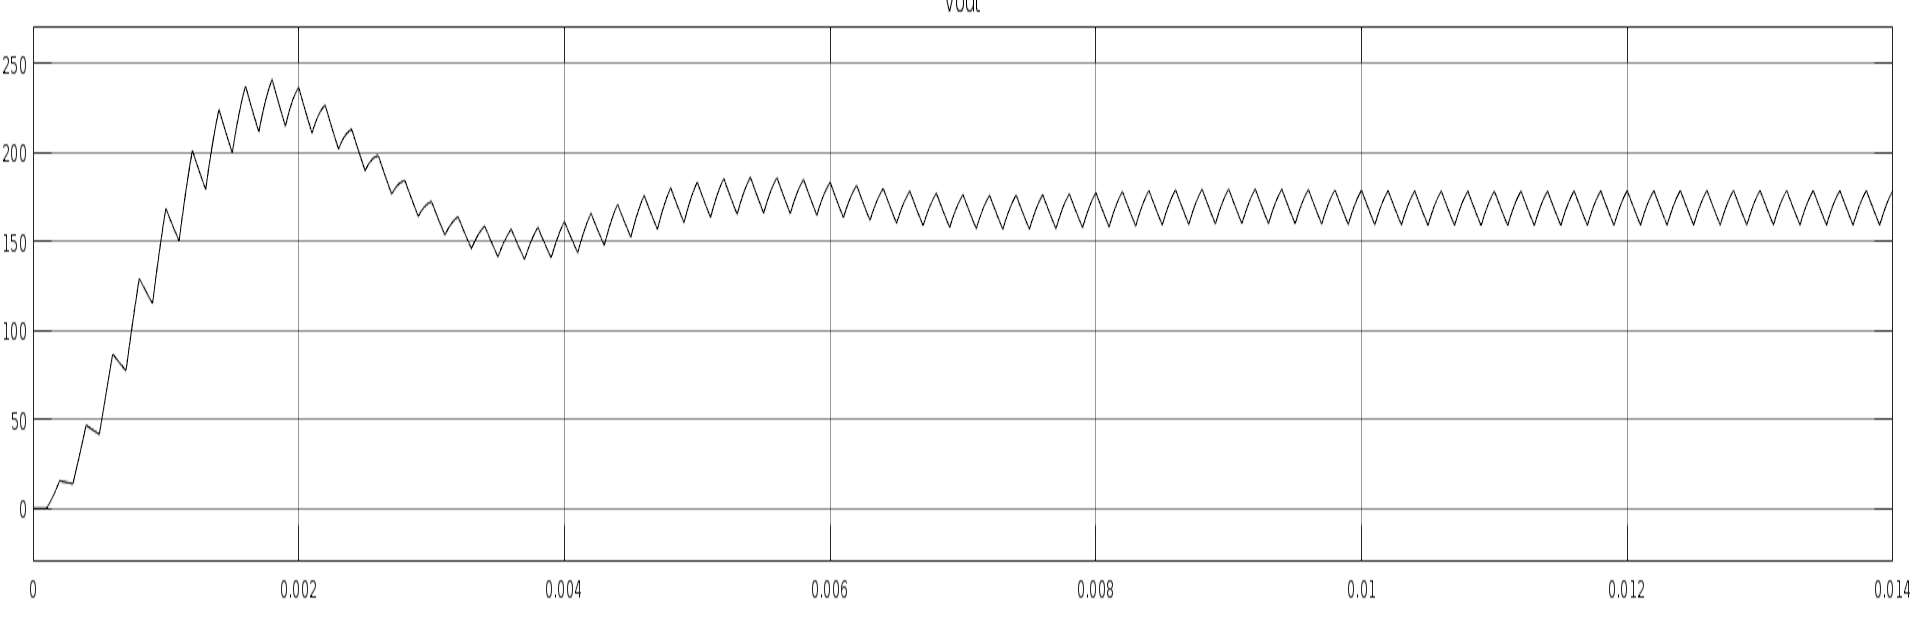
\includegraphics[scale=0.3]{measure_g05_snippet3.png}
\caption{результаты моделирования повышающего преобразователя в программе matlab: 
 частота переключения -- 5кГц,
коэффициент заполнения $\gamma=0.5$, $U_1=85$ В, $L=0.102$ Гн, $C=0.75$ мкФ, $R_\textcyrillic{нагрузки}=1157$ Ом}
	\label{matlab}
\end{figure}

\section*{Литература}
\renewcommand{\bibname}{}
\begin{thebibliography}{1} 
        \bibitem{Tsypkin}Цыпкин Я.З. Теория линейных импульсных систем ~М.: Государственное изд. физико-математической литературы 
                 1963. 968 с.  
\end{thebibliography}

\end{document}
